\documentclass{beamer} 
\usepackage{beamerthemesplit} 
\usepackage{wrapfig} 
\usepackage{verbatim} 
\usetheme{SPbGU} 
\usepackage{pdfpages} 
\usepackage{amsmath} 
\usepackage{cmap}
\usepackage{array} 
\usepackage[T2A]{fontenc} 
\usepackage[utf8]{inputenc} 
\usepackage[english,russian]{babel} 
\usepackage{indentfirst} 
\usepackage{amsmath} 
\usepackage{tikz} 
\usepackage{multirow} 
\usepackage[noend]{algpseudocode} 
\usepackage{algorithm} 
\usepackage{algorithmicx} 
\usetikzlibrary{shapes,arrows} 
\usepackage{fancyvrb} 
\usepackage{tikz} 
\usepackage{pgfplots} 
\usepackage{sidecap} 
\usepackage{soul}
\usepackage{xcolor}
\usepackage{tabu}
\usepackage{tikz}
\usetikzlibrary{calc}
\usepackage{zref-savepos}
\usepackage{colortbl}
\pgfplotsset{compat=1.9} 
\newtheorem{rutheorem}{Теорема} 
\newtheorem{ruproof}{Доказательство} 
\newtheorem{rudefinition}{Определение} 
\newtheorem{rulemma}{Лемма} 
\beamertemplatenavigationsymbolsempty 

\newcounter{NoTableEntry}
\renewcommand*{\theNoTableEntry}{NTE-\the\value{NoTableEntry}}

\newcommand*{\strike}[2]{%
	\multicolumn{1}{#1}{%
		\stepcounter{NoTableEntry}%
		\vadjust pre{\zsavepos{\theNoTableEntry t}}% top
		\vadjust{\zsavepos{\theNoTableEntry b}}% bottom
		\zsavepos{\theNoTableEntry l}% left
		\hspace{0pt plus 1filll}%
		#2% content
		\hspace{0pt plus 1filll}%
		\zsavepos{\theNoTableEntry r}% right
		\tikz[overlay]{%
			\draw
			let
			\n{llx}={\zposx{\theNoTableEntry l}sp-\zposx{\theNoTableEntry r}sp-\tabcolsep},
			\n{urx}={\tabcolsep},
			\n{lly}={\zposy{\theNoTableEntry b}sp-\zposy{\theNoTableEntry r}sp},
			\n{ury}={\zposy{\theNoTableEntry t}sp-\zposy{\theNoTableEntry r}sp}
			in
			(\n{llx}, \n{lly}) -- (\n{urx}, \n{ury})
			;
		}% 
	}%
}

\title[]{Поддержка расширенных контекстно-свободных грамматик в алгоритме синтаксического анализа Generalized LL} 
% То, что в квадратных скобках, отображается в левом нижнем углу. 
\institute[СПбГУ]{ Санкт-Петербургский Государственный Университет } 

% То, что в квадратных скобках, отображается в левом нижнем углу. 
\author[Горохоа Артем]{Горохов Артем} 
\date{19 апреля 2017} 

\begin{document} 
	
	\definecolor{red}{RGB}{255,0,0} 
	
	\begin{frame}
		\begin{center} 
			{\includegraphics[width=2.5cm]{pictures/SPbGU_Logo.png}} 
		\end{center}
		\titlepage
	\end{frame}

	\begin{frame}
		\begin{center} 
			{\includegraphics[width=12cm]{pictures/java_grammar.png}} 
		\end{center}
	\end{frame}

	\begin{frame} 
		\frametitle{Расширенные контекстно-свободные грамматики}
		\begin{center}
			{$\begin{aligned}
				S\ =&\ a\ M^* \\
				M\ =&\ a?\ (B\ K)^+ \\
				|&\ u\ B \\
				B\ =&\ c\ |\ \varepsilon
				\end{aligned}$}
		\end{center}
	\end{frame}
	
	\begin{frame}
		\frametitle{Результат преобразования в BNF}
		\begin{tabular}{c c}
		7 нетерминалов & 18 нетерминалов
		\\
		\multicolumn{2}{c}{
		\begin{columns}
			\begin{column}{6.1cm}
				\includegraphics[width=6cm]{pictures/java_before.png}
			\end{column}
			\begin{column}{.7cm}
				$ \Longrightarrow $
			\end{column}
			\begin{column}{5cm}
				\includegraphics[width=3.5cm]{pictures/java_after.png}
			\end{column}
	    \end{columns}
    }
        \end{tabular}
	\end{frame}

\begin{frame}
	\begin{center} 
		\only<1>{\includegraphics[width=12cm]{pictures/java_grammar.png}} 
		\only<2>{\includegraphics[width=12cm]{pictures/java_grammar_2.png}} 
	\end{center}
\end{frame}

	
	\begin{frame} 
		\frametitle{Существующие решения} 
		\begin{itemize}
			\item<1-> ANTLR, Yacc, Bison
			 \begin{itemize}
			 	\item<2-> Не могут использовать ECFG без преобразования
			 	\item<2-> Допускают только подклассы контекстно-свободных языков (LL(k), LR(k))
			 \end{itemize} 
			\item<3-> Работы о синтаксическом анализе ECFG
			\begin{itemize}
				\item<4-> Нет инструментов
				\item<4-> LL(k), LR(k)
			\end{itemize}
			\item<5-> \only<5-6>{Generalized LL}\only<7>{\textbf{Generalized LL}}
			\begin{itemize}
				\item<6-> Допускают произвольные CFG (включая неоднозначные)
				\item<6-> Не могут использовать ECFG без преобразований
			\end{itemize}
		\end{itemize}
	\end{frame}

\begin{frame}
	\frametitle{Биоинформатика}
	\begin{itemize}
		\item Множество задач, связанных с обработкой и пониманием биологических данных
		\item Одна из задач --- поиск организмов в метагеномных сборках
	\end{itemize}
\end{frame}

\begin{frame}
	\frametitle{Геном}
	\begin{itemize}
		\item Геном --- длинная последовательность нуклеотидов
		\item На деле строка над алфавитом \{A, C, G, U\}
	\end{itemize}
\end{frame}

\begin{frame}
	\frametitle{Получение данных}
	\begin{tabular}{p{5cm} p{7cm}}
		\begin{itemize}
			\item Из биологического материала читаются короткие строчки
			\item Эти кусочки склеиваются в более длинные строки
			\item Множество строчек --- сборка
			\item Данных очень много, поэтому строится граф, пути в котором содержат полученные строки
		\end{itemize}
		&
		\begin{figure}[b]
			\centering
			\includegraphics[width=6.5cm]{pictures/readsAssembly.png}  
		\end{figure}
	\end{tabular}
\end{frame}

\begin{frame}
	\frametitle{Метагеномная сборка}
	\begin{itemize}
		\item Изучаем набор генов всех микроорганизмов в образце
		\item Нужно уметь определять содержащиеся в сборке огранизмы
	\end{itemize}
\end{frame}

\begin{frame}
	\frametitle{Как ищем}
	\begin{tabular}{p{6cm} p{5cm}}
		\begin{itemize}
			\item Хочется понять что у нас в сборке
			\item Такие последовательности как тРНК, рРНК и др. позволяют провести классификацию организма
			\item У этих последовательностей есть вторичная структура, которая может быть описана КС-грамматикой
		\end{itemize}
		&
		\vspace{-1cm}
		\begin{figure}[b]
			\centering
			\includegraphics[width=5.2cm]{pictures/TRNA.png}
			\caption{Cтруктура тРНК}
		\end{figure}
	\end{tabular}  
\end{frame}

\begin{frame}
	\frametitle{YaccConstructor}
	\begin{itemize}
		\item В рамках проекта реализован алгоритм, основанный на алгоритме GLL
		\item Умеет решать задачу поиска линейных цепочек в графе, удовлетворяющих КС-грамматике
	\end{itemize}
\end{frame}

	\begin{frame} 
		\frametitle{Цель и задачи}
		Цель работы: разработать и реализовать модификацию алгоритма GLL, работающую с расширенными контекстно-свободными грамматиками, и проверить, как полученный алгоритм повлияет на производительность поиска структур, заданных с помощью контекстно-свободной грамматики, в метагеномных сборках.
		Для её достижения были поставлены следующие задачи:
		\begin{itemize}
			\item Выбрать или разработать подходящее представление ECFG
			\item Спроектировать структуру данных для представления леса разбора по ECFG
			\item Разработать алгоритм на основе Generalized LL, строящий лес разбора по ECFG
			\item Реализовать алгоритм в рамках проекта YaccConstructor
			\item Провести эксперименты и сравнение
		\end{itemize}
	\end{frame}

	\begin{frame} 
		\frametitle{Автоматы и ECFG}
		
		\begin{columns}
			\begin{column}{4cm}
				Грамматика $G_0$\\
				\vspace{10pt}
				$
				\begin{array}[b]{rl}
				S = a^{*} S\ b? \ | \ c \ \ \ \ \ \ \ \ \  \Longrightarrow
				\end{array}
				$
			\end{column}
			\begin{column}{3.3cm}
				RA для грамматики $G_0$\\
				\vspace{10pt}
				\includegraphics[width=2.5cm]{pictures/G0initialAutomaton.pdf}
			\end{column}
		\end{columns}
	\end{frame}

	\begin{frame} 
		\frametitle{Минимизация рекурсивных автоматов}
		\vspace{-12pt}
		\begin{center}
			%\begin{tabular}{c}
			{Грамматика $G_1$\\
			\vspace{5pt}
			$
			\begin{array}{rl}
			S =& K\ K\ K\ K\ K\ K \ |K\ a\ K\ K\ K\ K \\
			K =& S\ K\ |\ a\ K\ |\ a \\
			\end{array}
			$
			}
		    \\
		    \vspace{12pt}
		    Automaton for $G_1$
		    \\
		    \vspace{5pt}
		    {
				\includegraphics[width=7cm]{pictures/G1initial.pdf}
			}\\
			\vspace{8pt}
			Минимизированный автомат для $G_1$
			\\
			\vspace{5pt}
		    {
				\includegraphics[width=7cm]{pictures/G1automaton.pdf}
			}
		\end{center}
	\end{frame}
	
	\begin{frame} 
		\frametitle{Деревья вывода для рекурсивных автоматов}
		%\vspace{-40pt}
		\begin{columns}
			\begin{column}{3.7cm}
				%Grammar: $$ S : a^{+} S\ b? \ | \ c $$
				Вход: $$aacb$$ \\
				\vspace{10pt}
				Automaton: \\
				\vspace{5pt}
				\begin{center}
					\includegraphics[width=2cm]{pictures/G0minimizedAutomaton.pdf}
				\end{center}
			\end{column}
		
     		\begin{column}{6cm}
     			\ \ Деревья вывода:\\
     			\vspace{5pt}
     			\includegraphics[width=7cm]{pictures/G0trees.pdf}
			\end{column}
		
		\end{columns}
	\end{frame}
	
	\begin{frame} 
		\frametitle{SPPF для рекурсивных автоматов}
		\begin{columns}
			\begin{column}{5cm}
				%Grammar: $$ S : a^{+} S\ b? \ | \ c $$
				Вход: $$aacb$$ \\
				\vspace{10pt}
				Автомат: \\
				\vspace{5pt}
				\begin{center}
					\includegraphics[width=2cm]{pictures/G0minimizedAutomaton.pdf}
				\end{center}
			\end{column}
			\begin{column}{6cm}
				Shared Packed Parse Forest: \\
				\vspace{10pt}
				\only<1>{\includegraphics[width=5cm]{pictures/G0SPPF.pdf}}
				\only<2>{\includegraphics[width=5cm]{pictures/G0SPPF_1.pdf}}
				\only<3>{\includegraphics[width=5cm]{pictures/G0SPPF_2.pdf}}
				\only<4>{\includegraphics[width=5cm]{pictures/G0SPPF_3.pdf}}
			\end{column}
		\end{columns}
	\end{frame}
	
	\begin{frame} 
		\frametitle{Постоение леса разбора в оригинальном алгоритме}
		\begin{itemize}
			\item Очередь дескрипторов
			\item Дескриптор (G, i, U, T) однозначно определяет состояние процесса разбора
			\begin{itemize}
				\item G - \only<1>{позиция в грамматике}
						  \only<2>{\textbf{состояние в автомате}}
				\item i - позиция во входе
				\item U - узел стека разбора
				\item T - корень построенного леса разбора
			\end{itemize}
		\end{itemize}
		
	\end{frame}
	\begin{frame} 
		\frametitle{Пример постоения леса разбора в оригинальном алгоритме}
		\begin{columns}
			\begin{column}{5cm}
				Вход : \only<1-2>{$\ b c $}
						\only<3-7>{$\bullet\ b c $} 
						\only<8-11>{$b\bullet c $}
						\only<12->{$b c \bullet$} \\
				\vspace{15pt}
				Грамматика: \\
				\vspace{5pt}
				\only<1>{$$
					S = \ (a\ |\ b\ |\ S)\ c?
					$$}
				\only<2->{$
				\begin{array}{rl}
				S =&\only<3,6>{\bullet} \ a\ C\_opt \\
				|&\only<4,7>{\bullet} \ b\only<8>{\bullet}\ C\_opt \\
				|&\only<5>{\bullet} \ S\ C\_opt \\
				C\_opt =& \only<9>{\bullet} \varepsilon \ | \only<10-11>{\bullet} \ c \only<12>{\ \bullet}\\
				\end{array}
				$}
			\end{column}
			
			\begin{column}{5cm}
				\only<3->{
				\only<8>{\vspace{50pt}}
				\only<12>{\vspace{44pt}}
				\begin{center}Descriptors queue\\\end{center}
				\begin{tabu}{|[3pt]c|[3pt]}
					\only<10>{$C\_opt =\bullet c$, 1, \dots, \dots \\ \hline}
					\only<11->{\cellcolor{green!25}{$C\_opt =\bullet c$, 1, \dots, \dots} \\ \hline}
					\only<11->{\st{$C\_opt =\bullet  \varepsilon$, 1, \dots, \dots} \\ \hline}
					\only<9-10>{$C\_opt =\bullet  \varepsilon$, 1, \dots, \dots \\ \hline}
					\only<5-10>{$S =\bullet \ S\ C\_opt$, 0, \dots, \dots \\ \hline}
					\only<11->{\st{$S =\bullet \ S\ C\_opt$, 0, \dots, \dots} \\ \hline}
					\only<3-4>{$\ \ \ \ \ \ \ \ \ \ \ \ \ \ \ \ \ \ \ \ \ \ \ \ \ \ \ \ \ \ \ \ \ \ $ \\}
					%\strike{|[3pt]c|}{quux} & A & B \\
					\only<4-6>{$S =\bullet \ b\ C\_opt$, 0, \dots, \dots \\ \hline}
					\only<7-10>{\cellcolor{green!25}{$S =\bullet \ b\ C\_opt$, 0, \dots, \dots} \\ \hline}
					\only<11->{\st{$S =\bullet \ b\ C\_opt$, 0, \dots, \dots} \\ \hline}
					\only<3>{$\ \ \ \ \ \ \ \ \ \ \ \ \ \ \ \ \ \ \ \ \ \ \ \ \ \ \ \ \ \ \ \ \ \ $ \\}
					\only<3-5>{$S =\bullet \ a\ C\_opt$, 0, \dots, \dots}
					\only<6>{\cellcolor{green!25}{$S =\bullet \ a\ C\_opt$, 0, \dots, \dots}}
					\only<7->{\st{$S =\bullet \ a\ C\_opt$, 0, \dots, \dots}}
				\end{tabu}
			}
		
			\only<8>{
				\vspace{20pt}
				\begin{center}
					\only<8>{\includegraphics[width=2cm]{pictures/example_trees_b.pdf}}
				\end{center}				
			}
			\only<12>{
				\begin{center}
					\includegraphics[width=2cm]{pictures/example_trees.pdf}
				\end{center}				
			}
			\end{column}
		    
		\end{columns}
	\end{frame}

	\begin{frame} 
		\frametitle{Input processing}
		\begin{columns}
			\begin{column}{5cm}
				Input : $\only<1>{\ \ }\only<2->{\bullet} \ b c $ \\
				\vspace{15pt}
				Automaton : \\
				\vspace{5pt}
				\only<1>{\includegraphics[width=5cm]{pictures/G2.pdf}}
				\only<2>{\includegraphics[width=5cm]{pictures/G2_1.pdf}}
				\only<3>{\includegraphics[width=5cm]{pictures/G2_2.pdf}}
			\end{column}
			\begin{column}{3cm}
				%\only<3>{\vspace{50pt}}
				\begin{center}
				\only<2>{
				Descriptors queue\\
				\begin{tabu}{|[3pt]c|[3pt]}
					\only<2->{$S$, 0, \dots, \dots}
				\end{tabu}
				}
				\only<3>{
					\includegraphics[width=4cm]{pictures/example_trees_auto.pdf}
				}
				\end{center}
			\end{column}
		\end{columns}
	\end{frame}
	
	\begin{frame} 
		\frametitle{Evaluation}
		\begin{center}
		\vspace{-10pt}
		Grammar $G_1$\\
		\vspace{6pt}
		$
		\begin{array}{rl}
		S =& K\ K\ K\ K\ K\ K \ | K\ a\ K\ K\ K\ K \\
		K =& S\ K\ |\ a\ K\ |\ a \\
		\end{array}
		$
		\\
		\vspace{10pt}
		RA for grammar $G_1$
		\\
		\vspace{6pt}
		\includegraphics[scale=.5]{pictures/G1automaton.pdf}
		\\
		\vspace{7pt}
		Experiment results for input $a^{40}$
		\\
		\vspace{2pt}
		\begin{tabular}{ | c | c | c | c | c | }
			\hline
			\multirow{2}{*}[-1ex]{} &\multicolumn{3}{c|}{Memory usage} & \multirow{2}{*}[-1ex]{Time,sec} \\
			\cline{2-4}
             &  Descriptors & Stack Edges & SPPF Nodes &    \\ \hline
			Grammar  &  7,940        & 6,974      & 111,127,244 & 81 \\ \hline
		     RA &  5,830        & 4,234      & 74,292,078  & 54 \\ \hline \hline
			Ratio   &  27$\%$       & 39$\%$     & 33 $\%$ & 35 $\%$    \\ \hline
		\end{tabular}
		\end{center}
	\end{frame}
	
	\begin{frame} 
		\frametitle{Applicability} 
		\begin{center}
		\vspace{-40pt}
		Graph parsing: all input strings in one graph
		\begin{columns}
			\begin{column}{1cm}
			\end{column}
			\begin{column}{1cm}
				\begin{center}
				$abcd$ \\ 
				$abfd$
				\end{center}
			\end{column}
			\begin{column}{.7cm}
				\\
				$ \Longrightarrow $
			\end{column}
			\begin{column}{6cm}
			\includegraphics[width=6cm]{pictures/graph.pdf}
			\end{column}
		\end{columns}
		\vspace{40pt}
		Graph parsing results
		\begin{tabular}{ | c | c | c | c | c | }
			\hline
			\multirow{2}{*}[-1ex]{} &\multicolumn{3}{c|}{Memory usage} & \multirow{2}{*}[-1ex]{Time, min } \\
			\cline{2-4}
			             &  Descriptors & Stack Edges & Stack Nodes &   \\ \hline
			Grammar  &  21,134,080       & 7,482,789      & 2,731,529      & 02.26  \\ \hline
			RA &  9,153,352        &  2,792,330     & 839,148        & 01.25  \\ \hline \hline
			Ratio   &  57$\%$       & 63$\%$     & 69 $\%$    &  45 $\%$ \\ \hline
		\end{tabular}
		\end{center}
	\end{frame}

	\begin{frame} 
		\frametitle{Results}
		\begin{itemize}
			\item GLL for extended context-free grammars
			\begin{itemize}
				\item For linear input
				\item Graph input			
			\end{itemize}
			\item Started evaluation on real graphs
		\end{itemize}
		
	\end{frame}
\end{document}